\textnormal{
\begin{itemize} 
\item{The the first SQL statement used to query the data: }
Here is a simple query to start off:\\
	SELECT * \\FROM Part P \\WHERE P.PName = "Intel Computer Stick" \\    AND P.Pid = 1337\\
	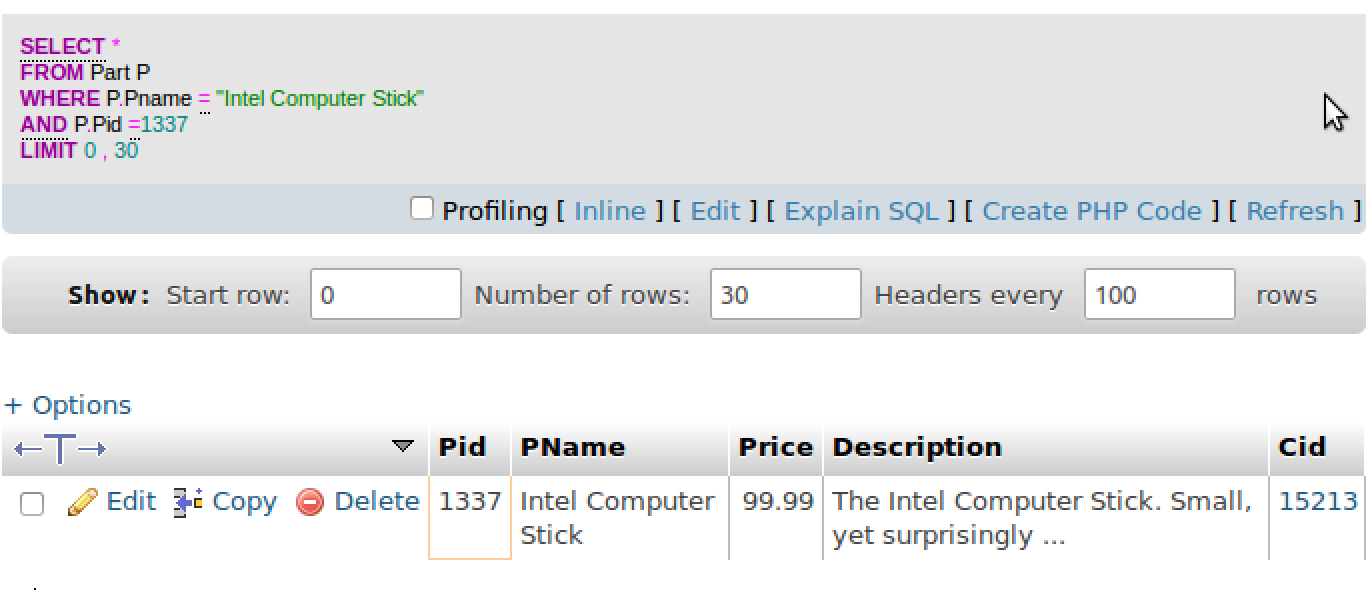
\includegraphics[width=\columnwidth]{Query1.png} 
\item{The tables taking part in the query statement (table names and headers): }
	 \begin{itemize} 
	 \item{The name of the first table taking part in the query: }
	 Part table
	  \item{The header of the table  (all attributes): }
	  Pid, PName, Price, Description, Cid
	  \item{The attributes of the table taking part in the query: }
	  PName and Pid
	 \end{itemize}
\item{The the second SQL statement used to query the data: }
	SELECT * \\FROM Part P, Buys B\\WHERE P.Pid = B.Pid\\
	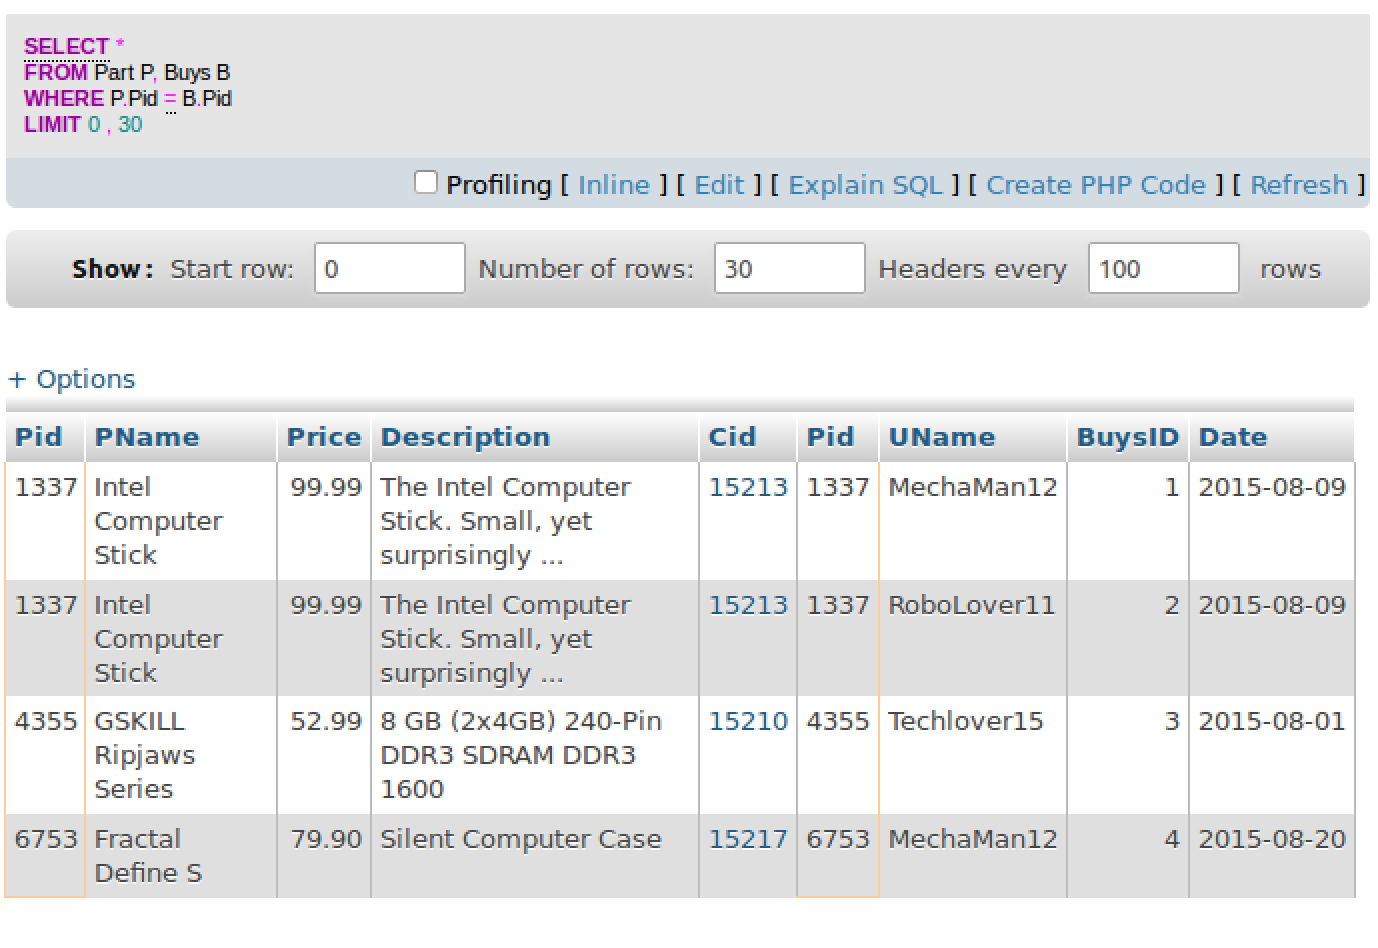
\includegraphics[width=\columnwidth]{Query2.png} 
\item{The tables taking part in the query statement (table names and headers): }
	 \begin{itemize} 
	 \item{The name of the tables taking part in the query: }
	 Part and Buys table
	  \item{The header of the table  (all attributes): }
	  Part: Pid, PName, Price, Description, Cid \\
	  Buys: Pid, UName, BuysID, Date
	  \item{The attributes of the table taking part in the query: }
	   Pid
	 \end{itemize}
	 \item{The the third SQL statement used to query the data: }
	SELECT * \\FROM Part P, Review R\\WHERE R.Rating >= 8 \\ AND P.Pid = R.Pid\\
	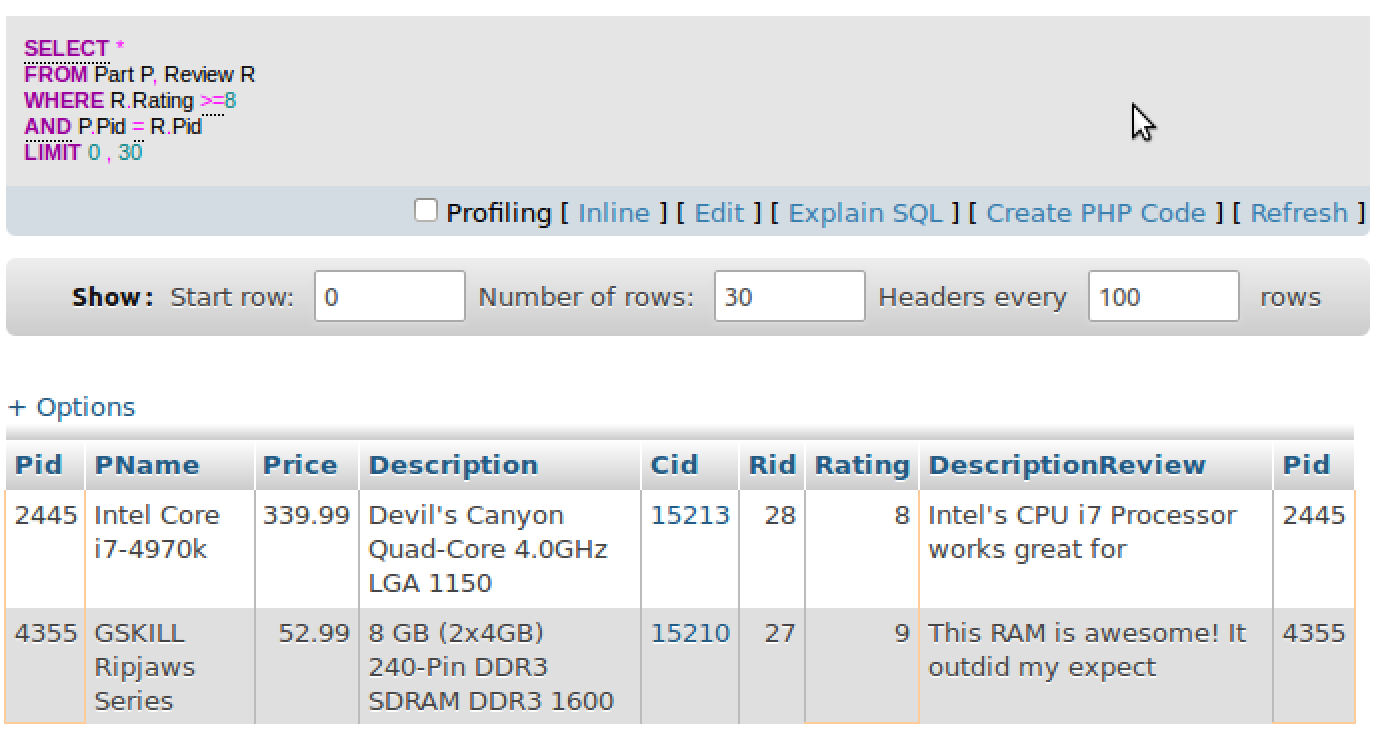
\includegraphics[width=\columnwidth]{Query3.png} 
\item{The tables taking part in the query statement (table names and headers): }
	 \begin{itemize} 
	 \item{The name of the tables taking part in the query: }
	 Part and Review table
	  \item{The header of the table  (all attributes): }
	  Part: Pid, PName, Price, Description, Cid \\
	  Review: Pid, Rid, Rating, Review Description
	  \item{The attributes of the table taking part in the query: }
	   Pid, rating
	 \end{itemize}
	 \item{The the fourth SQL statement used to query the data: }
	SELECT S.SName, P.PName \\FROM Seller S, Part P\\WHERE P.Price >= 99.99\\
	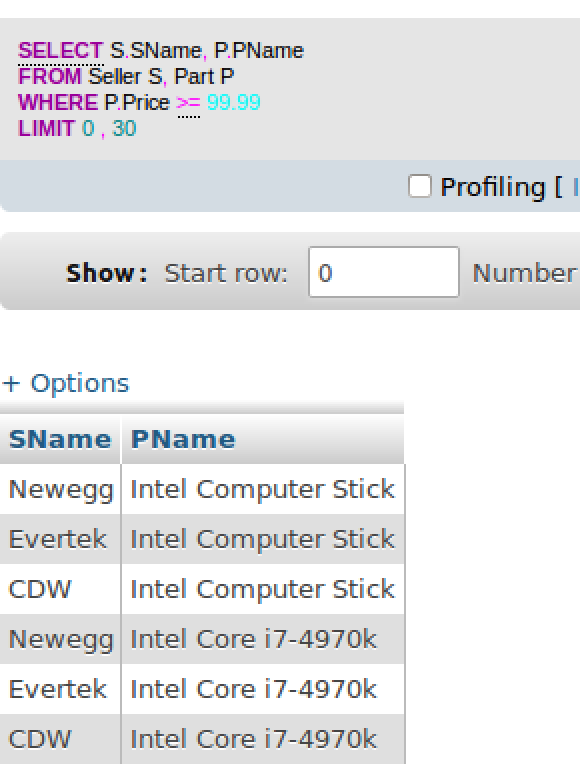
\includegraphics[width=\columnwidth]{Query4.png} 
\item{The tables taking part in the query statement (table names and headers): }
	 \begin{itemize} 
	 \item{The name of the tables taking part in the query: }
	 Seller and Part tables
	  \item{The header of the table  (all attributes): }
	  Part: Pid, PName, Price, Description, Cid \\
	  Seller: Sid, SName
	  \item{The attributes of the table taking part in the query: }
	   SName and PName
	 \end{itemize}
	 \item{The the fifth SQL statement used to query the data: }
	SELECT L.Lid \\FROM Seller S, Location L\\WHERE S.SName = ''Newegg'' OR S.SName = ''Evertek'' AND S.Sid = 5250\\
	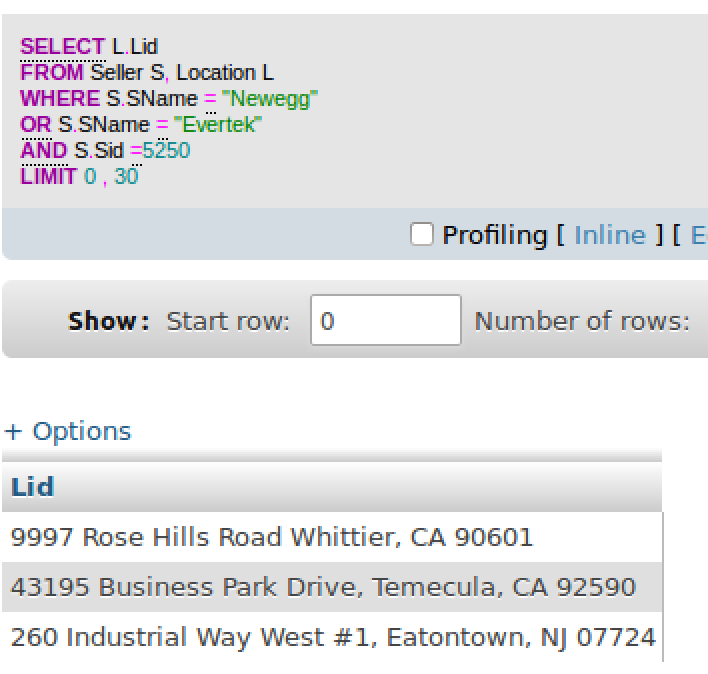
\includegraphics[width=\columnwidth]{Query5.png} 
\item{The tables taking part in the query statement (table names and headers): }
	 \begin{itemize} 
	 \item{The name of the tables taking part in the query: }
	 Seller and Location table
	  \item{The header of the table  (all attributes): }\\
	  Location: Lid \\
	  Seller: Sid, SName
	  \item{The attributes of the table taking part in the query: }
	   Lid
	 \end{itemize}
\item{}
	The error messages popping-up when users access and/or updates are denied (along with explanations and examples):
	\begin{itemize} 
	\item{The first error message: }
	\\CREATE command denied to user Account User
		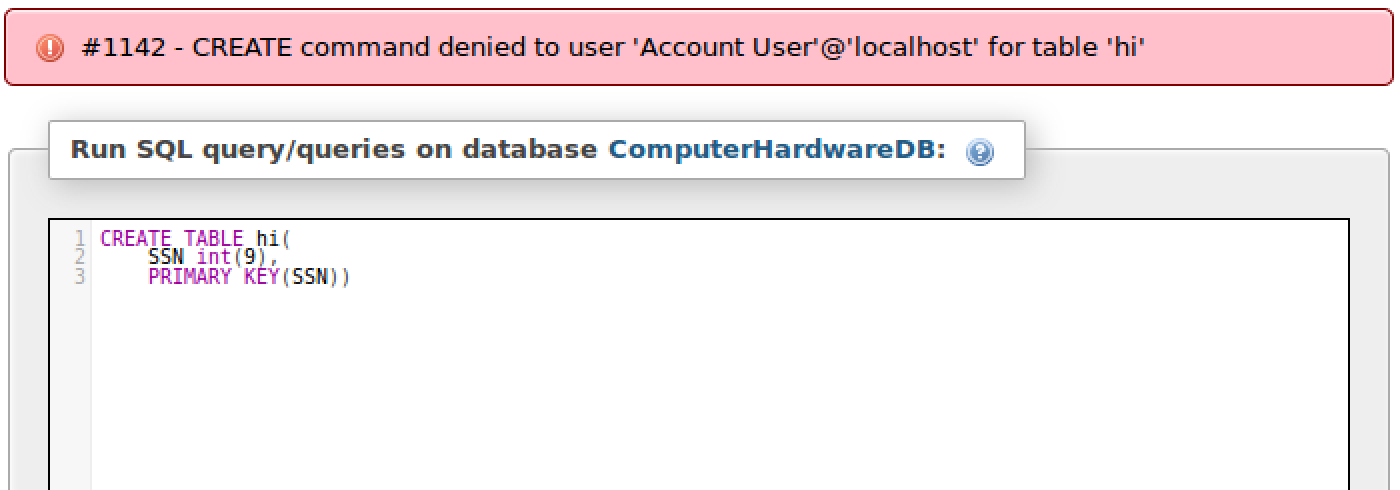
\includegraphics[width=\columnwidth]{Access1.png}
	\item{The error message explanation (upon which violation does it take place): }
	The user does not have the access rights for creating a table. 
	\item{The error message example according to user(s) scenario(s): }
	This account user accessing the Computer Hardware DB tried creating a table in the database. Account users, however, do not have access rights to do so. This account user must have mixed up his command with INSERT, a command which Account users are allowed access when inserting a rating and description review for the Reviews entity.\\
	Example:\\
	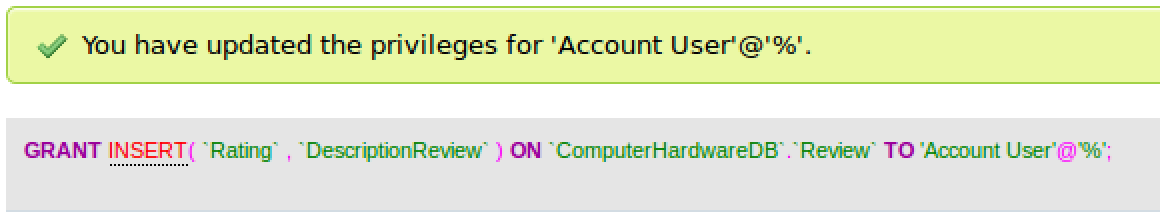
\includegraphics[width=\columnwidth]{Access2-1.png}
	 \end{itemize}
	\begin{itemize} 
	\item{The second error message: }
	\\INSERT command denied to user Guest User
		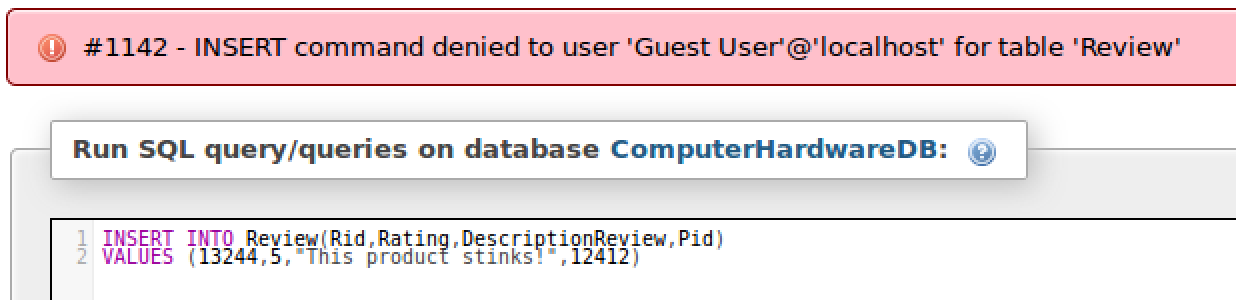
\includegraphics[width=\columnwidth]{Access2-2.png}
	\item{The error message explanation (upon which violation does it take place): }
	The user does not have the access rights for inserting into the database. 
	\item{The error message example according to user(s) scenario(s): }
	This guest user accessing the Computer Hardware DB tried inserting into the Review entity. Guest users, however, do not have access rights to do so. Guest user cannot write reviews or rate reviews like account users.
	 \end{itemize}
	 \begin{itemize} 
	\item{The third error message: }
	\\ALTER command denied to user Account User
		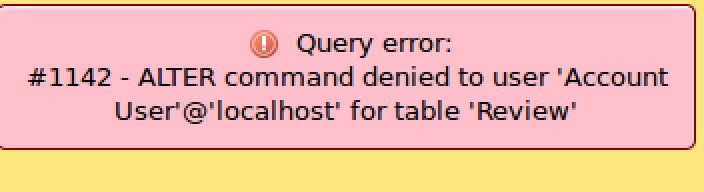
\includegraphics[width=\columnwidth]{Access3.png}
	\item{The error message explanation (upon which violation does it take place): }
	The user does not have the access rights for altering a table in the database. 
	\item{The error message example according to user(s) scenario(s): }
	This account user accessing the Computer Hardware DB tried to alter a table in the database. Account users, however, do not have access rights to do so. Account user cannot alter pre-existing attribute specifications in a table.
	 \end{itemize}
	 	 \begin{itemize} 
	\item{The fourth error message: }
	\\DELETE command denied to user Seller User
		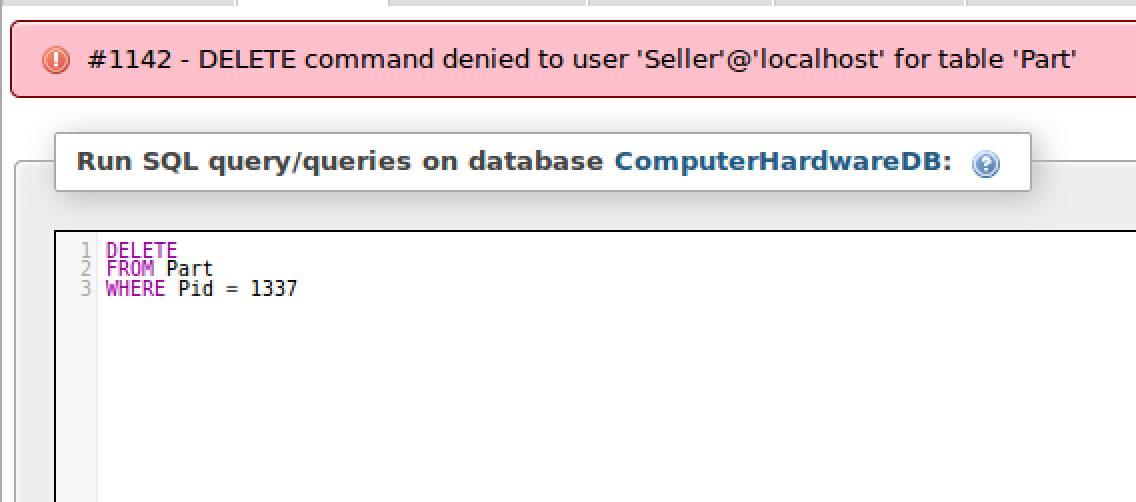
\includegraphics[width=\columnwidth]{Access4.png}
	\item{The error message explanation (upon which violation does it take place): }
	The user does not have the access rights for deleting information from a table in the database. 
	\item{The error message example according to user(s) scenario(s): }
	This seller accessing the Computer Hardware DB tried to delete a Pid from a table in the database. Seller users should not have access rights for deleting product information on a company's part. Only Company users should be able to remove their own information on a given part.
	 \end{itemize}
	 \begin{itemize} 
	\item{The fifth error message: }
	\\DROP command denied to user Company User
		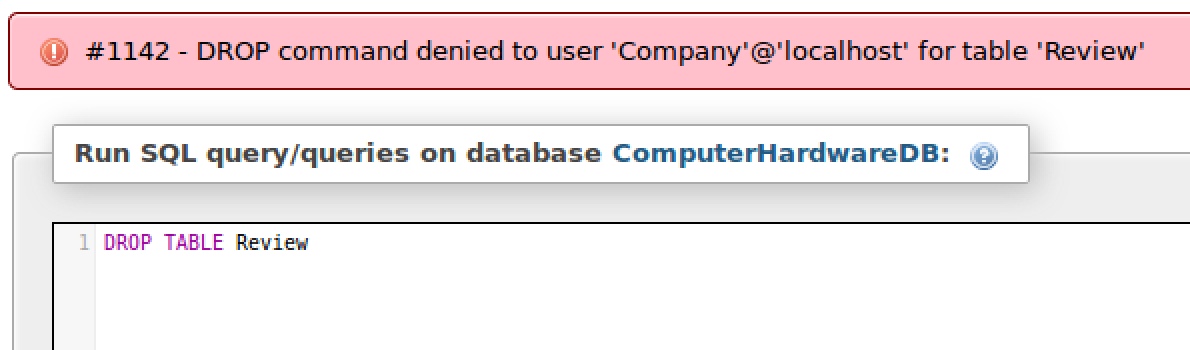
\includegraphics[width=\columnwidth]{Access5.png}
	\item{The error message explanation (upon which violation does it take place): }
	The user does not have the access rights for dropping an entire table from the database.
	\item{The error message example according to user(s) scenario(s): }
	This company user accessing the Computer Hardware DB tried to drop the Review table from the database. Company users, as well as all users of the database (with the exception of the DBA) should not have access rights for dropping entire tables from the database. The company user may have wanted to delete a review on their product that an account user did not like. Although it is frustrating to see bad reviews on a product one may have created, a prestigious company such as Intel should not take it to heart and rather learn from their potential falters. Ultimately, company users cannot and should not drop review information on their products.
	 \end{itemize}
\item{}
	The error messages corresponding to the integrity constraints violations (along with explanations and examples).
	\begin{itemize} 
	\item{The first error message: }
	Duplicate entry '4124' for key 'PRIMARY'\\
	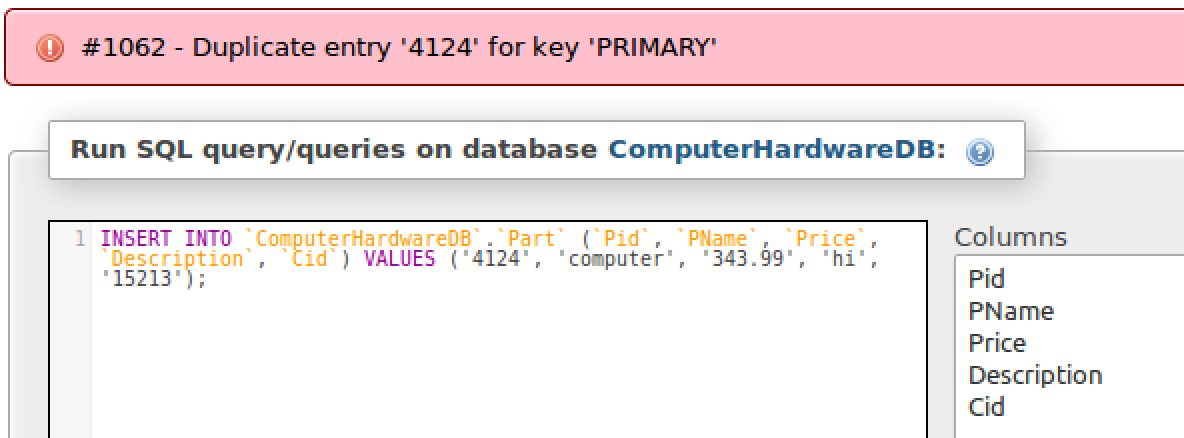
\includegraphics[width=\columnwidth]{integrity1.png}
	\item{The error message explanation (upon which violation does it take place): }
	When trying to INSERT a duplicate primary key for Pid, the system stops the command with a duplicate primary key constraint.  
	\item{The error message example according to user(s) scenario(s): }
	In order to ensure that changes made to the database do not result in loss of data and consistency, our database holds PRIMARY keys. These keys (such as Pid) allow our products in Part to be unique and have individual characteristics from all parts being added to the database. In the case if a seller tried to INSERT a duplicate part by accident in their retail system, the database system would catch it and save the seller time and money trying to find the root cause that is throwing off their inventory calculations. Having duplicate part ids can most definitely throw off a inventory database, and it is accounted for in our database.
	 \end{itemize}
	 	\begin{itemize} 
	\item{The second error message: }
	Cannot delete or update a parent row: a foreign key constraint fails\\
	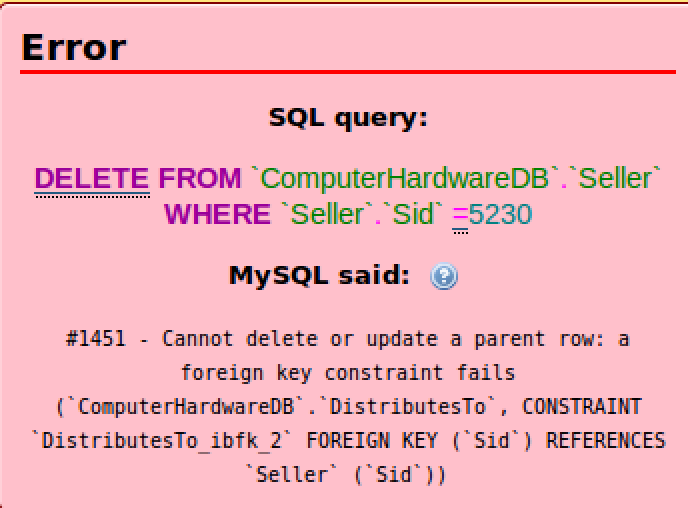
\includegraphics[width=\columnwidth]{integrity2.png}
	\item{The error message explanation (upon which violation does it take place): }
	When trying to DELETE a seller tuple from the database, a FOREIGN key constraint is thrown.
	\item{The error message example according to user(s) scenario(s): }
	In order to ensure that changes made to the database do not result in loss of data and consistency, our database holds FOREIGN keys. These keys allow our tables and entities within the database to be interconnected. In this example regarding the error message above, a person using the database, most likely a seller user, tried to delete their seller information from the database. This violates the database because information regarding seller id (Sid) is already linked to Companies through relation Manufactures as well as Part through relation SoldBy. This would throw off the database entries for multiple entities and relationships since they are all connected through use of foreign keys.
	 \end{itemize}
\item{}
	The error messages corresponding to the data range constraints violations (along with explanation).
	\begin{itemize} 
	\item{The first error message: }
	Column 'Pid' cannot be null\\
	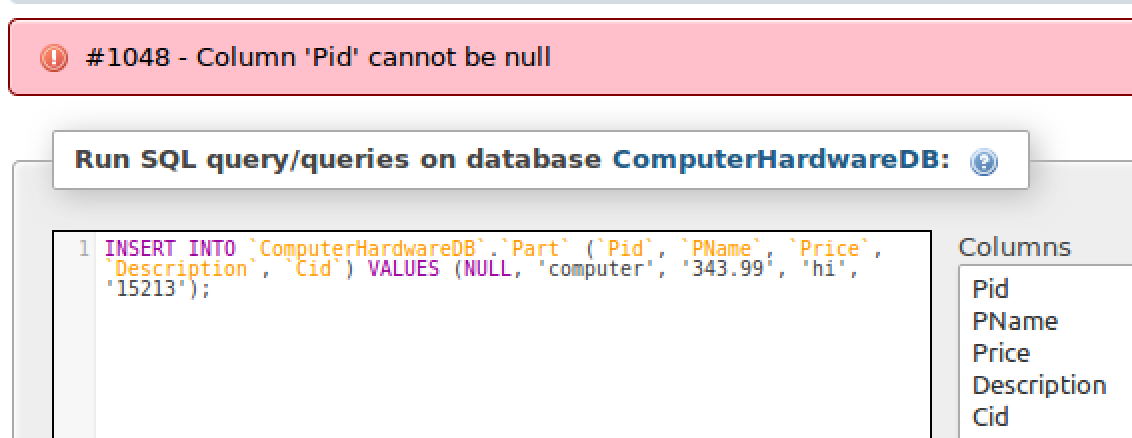
\includegraphics[width=\columnwidth]{datarange1.png}
	\item{The error message explanation (upon which violation does it take place): }
	For each PRIMARY key in the database, the value of it cannot be NULL. This would allow no uniqueness for an entity if it were given a NULL value. 
	\item{The error message example according to user(s) scenario(s): }
	An example where this error message might arise could be when a seller does not know the product id (Pid) initially but wants to insert its price, description and name. The seller cannot include NULL as information for Pid because it is a PRIMARY key. There would be no way of referencing that part if it was given a NULL value. 
	 \end{itemize}
	 	\begin{itemize} 
	\item{The second error message: }
	Out of range value for column 'Price' at row 1\\
	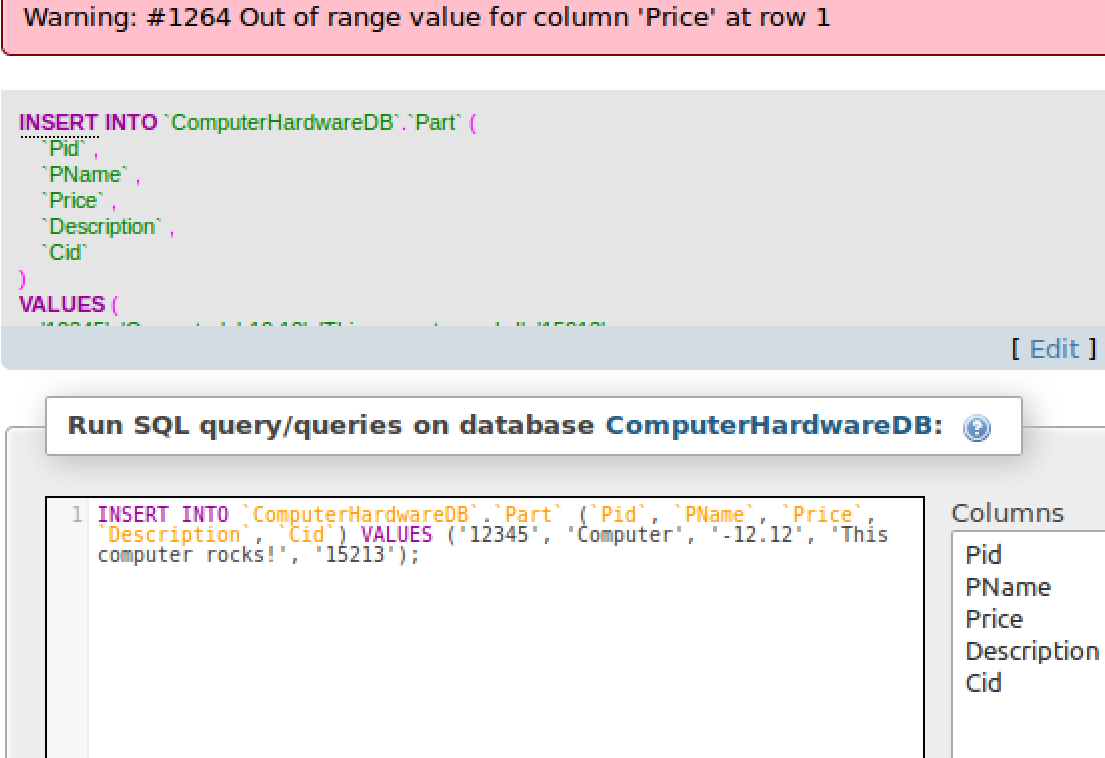
\includegraphics[width=\columnwidth]{datarange2.png}
	\item{The error message explanation (upon which violation does it take place): }
	For INT and FLOAT values in the database, they must be regarded as UNSIGNED values. There should be no negative values inserted into the database. 
	\item{The error message example according to user(s) scenario(s): }
	Most likely, the seller selling this part made a typo in the computer hardware database. A price cannot and should not be listed as a negative float value. 
	 \end{itemize}
\begin{itemize} 
	\item{The third error message: }
	Data truncated for column 'PName' at row 1\\
	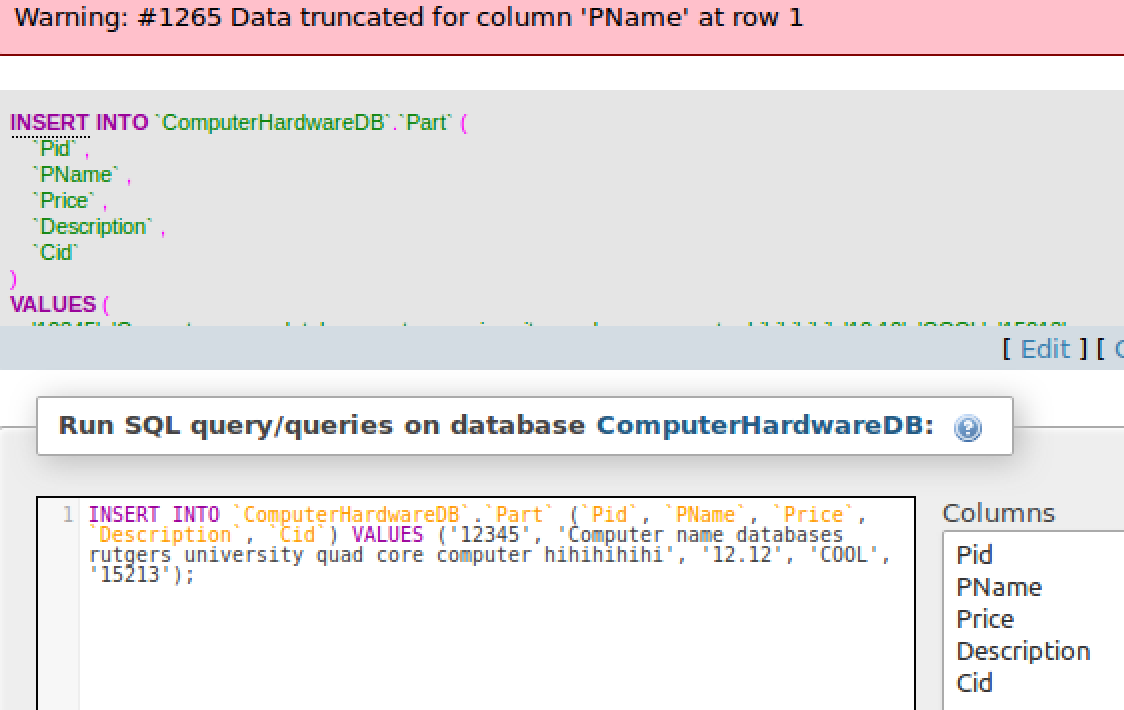
\includegraphics[width=\columnwidth]{datarange3.png}
	\item{The error message explanation (upon which violation does it take place): }
	For each product name in the Part entity, there is a limit to how long a PName can be. The error is throw because the PName is longer than varchar(30).
	\item{The error message example according to user(s) scenario(s): }
	For all varchar fields in the database, there is a certain limit to the amount of characters one can type for that attribute. This data-range constraint is to allow concise descriptions of each product name. We want to create a simple yet effective environment for our account users and guest users, and by making product descriptions clear and concise, we can achieve this. The database will automatically truncate the data if too long, hinting this to the seller/company to fix and alter immediately. 
	 \end{itemize}
\begin{itemize} 
	\item{The fourth error message: }
	Out of range value for column 'Price' at row 1\\
	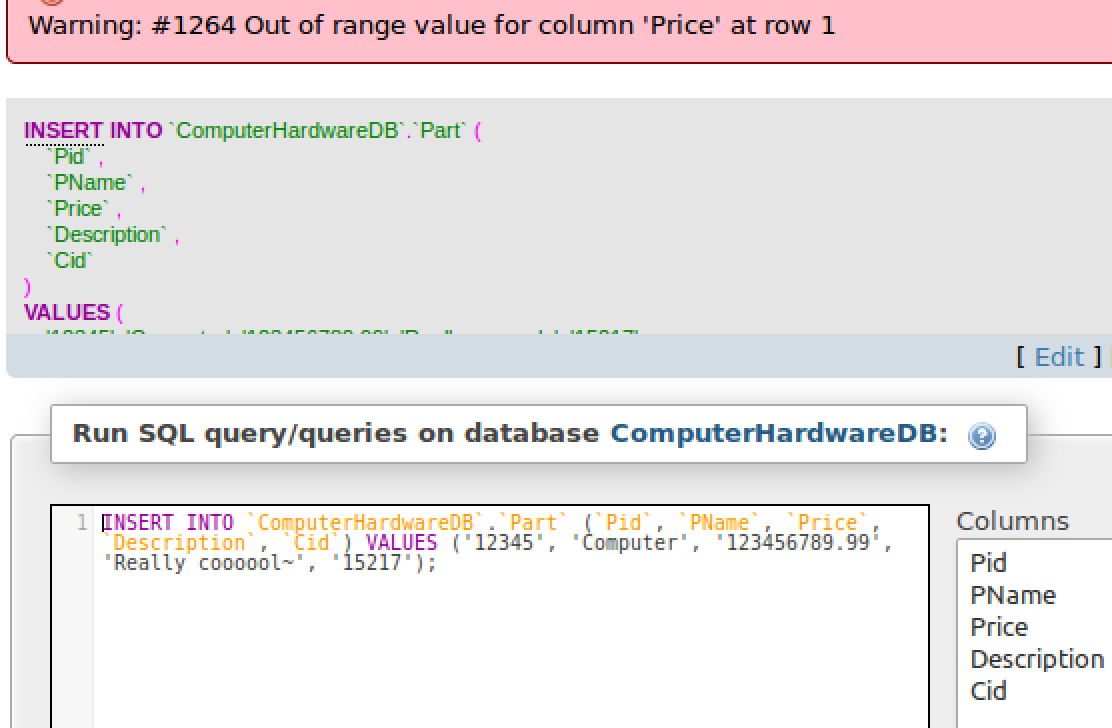
\includegraphics[width=\columnwidth]{datarange4.png}
	\item{The error message explanation (upon which violation does it take place): }
	The price of a product cannot exceed one million dollars in our database. Data that is larger than the specified data type will cause issues if not notified and dealt with immediately. We have accounted for this by adding a data-range constraint for the price field in the part entity through use of float(6,2). 
	\item{The error message example according to user(s) scenario(s): }
	 An example where this error might be thrown is when a seller lists the price of a part to be that greater than 999999.99. We do not want to deal with products greater than this value because it is simply a lot of money to deal with and there lies a lot more pressure on the database to keep the integrity and security of each transaction. If our database were to go through increased enhances involving data and transaction security, we would most definitely deal with such a fit. 
	 \end{itemize}
\item{The header of the views created in order to facilitate data accesses:}
\begin{itemize} 
	\item{The first view created: }\\
	Selects to view the part name, description, price, rating and description review.
	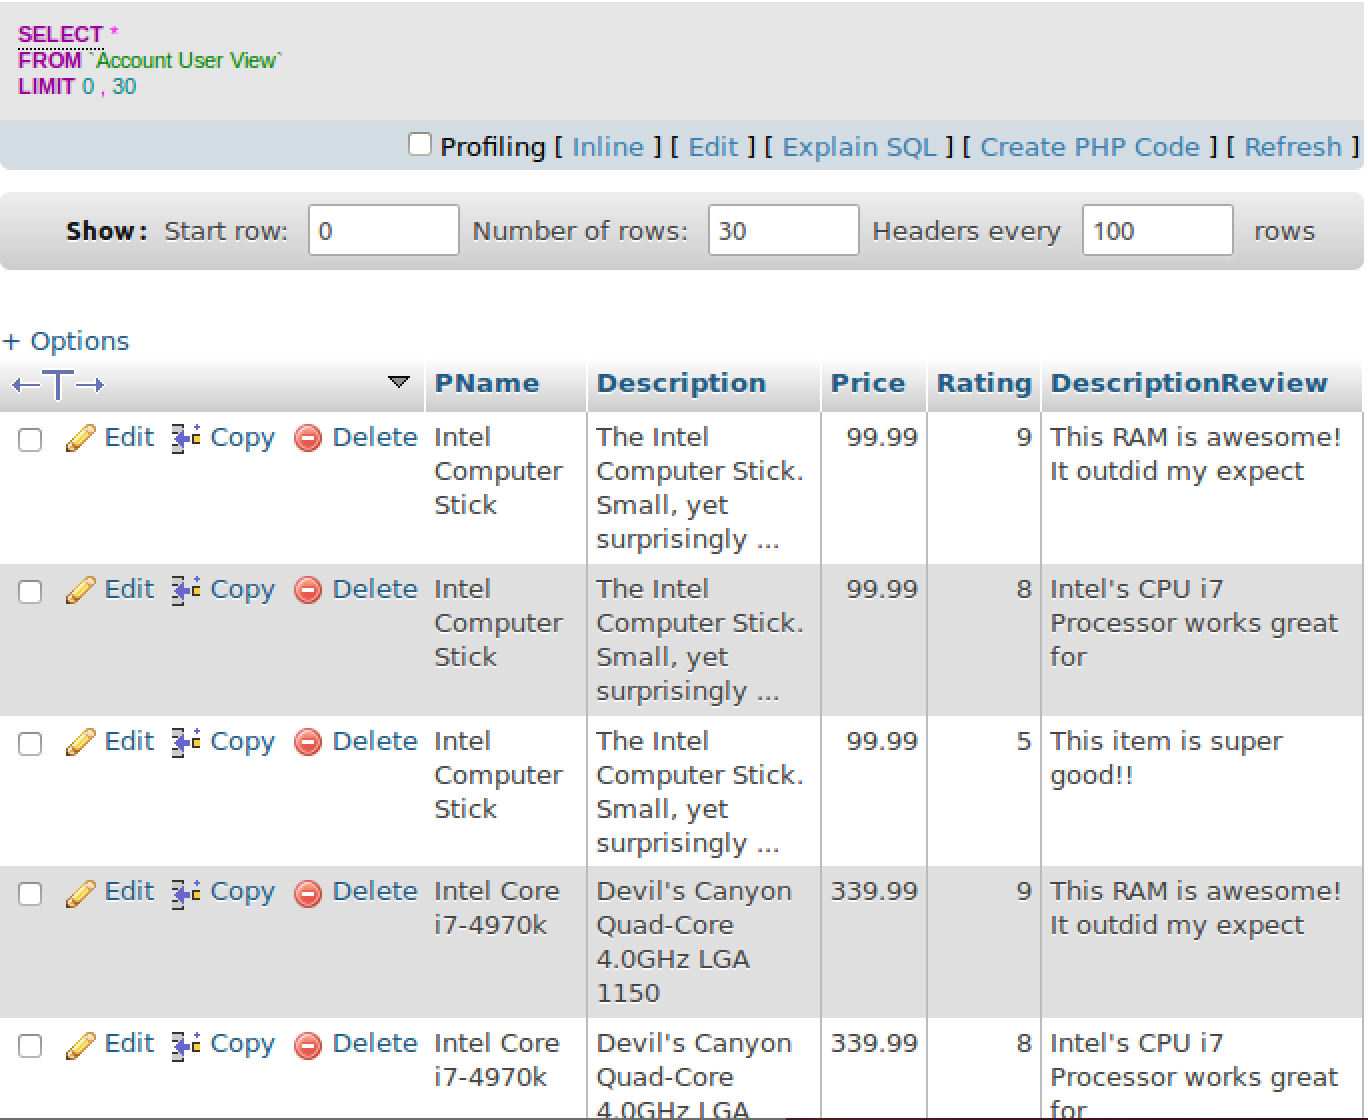
\includegraphics[width=\columnwidth]{view1.png}
	\item{The view justification: }
	This view was created with the Account User in mind. In order to make it simple for account users to make their purchase decisions, we created a view that shows all information regarding each part as well as reviews and ratings on that part. 
	\item{The tables taking part in the view and the specific attributes taking part in the view: }
	\begin{itemize} 
		\item{The table names: }
		Part and Review tables.
		\item{The table headers (all attributes): }\\
		Part: Pid, PName, Description, Price, Cid\\
		Review: Rid, Rating, DescriptionReview, Pid
		\item{The table attributes that take part in the view: }
		Part: PName, Description, Price\\
		Review: Rating, DescriptionReview
	\end{itemize}
	\item{The SQL statement used for creating the view: }
	SELECT P.Pname, P.Description, P.Price, R.Rating, R.DescriptionReview\\
	FROM Part P, Review R\\
%	\item{The trigger built upon those views (if any): }
%	Please insert the triggers as follows.
%	\begin{itemize} 
%		 \item{The trigger: }
%		Please insert the trigger in here.
%		 \item{The trigger justification (explanation, correlating it to user scenario(s)): }
%		Please insert the justification in here.
 %	\end{itemize}
 %	Please repeat for every trigger existing in the view.
\end{itemize}
\begin{itemize} 
	\item{The second view created: }\\
	Selects to view all of Intel's seller distributors of their products.\\
	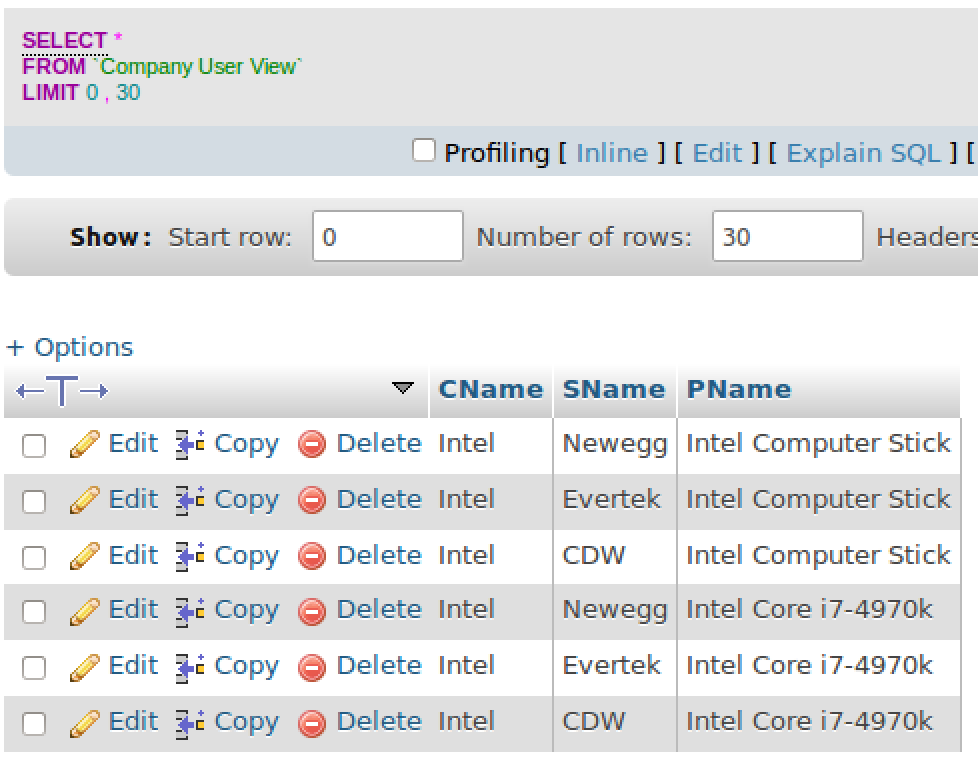
\includegraphics[width=\columnwidth]{view2.png}
	\item{The view justification: }
	This view was created with the Company User in mind. In order to keep track of their distribution of products, companies can create a view that allows them to see products they are currently distributing to different sellers.
	\item{The tables taking part in the view and the specific attributes taking part in the view: }
	\begin{itemize} 
		\item{The table names: }
		Company, Seller and Part tables.
		\item{The table headers (all attributes): }\\
		Company: Cid, CName\\
		Part: Pid, PName, Description, Price, Cid\\
		Seller: Sid, SName
		\item{The table attributes that take part in the view: }
		Company: CName\\
		Part: PName\\
		Seller: SName
	\end{itemize}
	\item{The SQL statement used for creating the view: }
	SELECT C.CName, S.SName, P.PName\\
	FROM Company C, Seller S, Part P\\
	WHERE C.CName = ''Intel'' AND C.Cid = P.Cid
%	\item{The trigger built upon those views (if any): }
%	Please insert the triggers as follows.
%	\begin{itemize} 
%		 \item{The trigger: }
%		Please insert the trigger in here.
%		 \item{The trigger justification (explanation, correlating it to user scenario(s)): }
%		Please insert the justification in here.
 %	\end{itemize}
 %	Please repeat for every trigger existing in the view.
\end{itemize}
%Please, in case you have more than one view, repeat that pattern for each view.
\end{itemize}
}
